%for a more compact document, add the option openany to avoid
%starting all chapters on odd numbered pages
\documentclass[12pt,openany]{cmuthesis}

% This is a template for a CMU thesis.  It is 18 pages without any content :-)
% The source for this is pulled from a variety of sources and people.
% Here's a partial list of people who may or may have not contributed:
%
%        bnoble   = Brian Noble
%        caruana  = Rich Caruana
%        colohan  = Chris Colohan
%        jab      = Justin Boyan
%        josullvn = Joseph O'Sullivan
%        jrs      = Jonathan Shewchuk
%        kosak    = Corey Kosak
%        mjz      = Matt Zekauskas (mattz@cs)
%        pdinda   = Peter Dinda
%        pfr      = Patrick Riley
%        dkoes = David Koes (me)

% My main contribution is putting everything into a single class files and small
% template since I prefer this to some complicated sprawling directory tree with
% makefiles.

% some useful packages
\usepackage{times}
\usepackage{fullpage}
\usepackage{graphicx}
\usepackage{amsmath}
\usepackage[numbers,sort]{natbib}
\usepackage[backref,pageanchor=true,plainpages=false, pdfpagelabels, bookmarks,bookmarksnumbered,
%pdfborder=0 0 0,  %removes outlines around hyper links in online display
]{hyperref}
\usepackage{subfigure}
\usepackage{comment}
\usepackage{url}
\usepackage{subfigure}
\usepackage{color}
\usepackage{ifthen}
\usepackage{framed}
\usepackage{multirow}
\usepackage{color,soul,xspace}
\usepackage{epsfig}
\usepackage{makecell}
\usepackage{booktabs}

\newenvironment{captiontext}{%
   \vspace{-0.1in}\begin{center}%
     \begin{minipage}{0.9\linewidth}%
       \renewcommand{\baselinestretch}{0.9}%
         \small}%
   {\renewcommand{\baselinestretch}{1.0}%
      \end{minipage}%
      \end{center}}

% Abbreviations
\newcommand{\lc}[1]{\lowercase{#1}}
\newcommand{\uc}[1]{\uppercase{#1}}
\newcommand{\xc}[1]{\small\sc #1}


% Approximately 1" margins, more space on binding side
%\usepackage[letterpaper,twoside,vscale=.8,hscale=.75,nomarginpar]{geometry}
%for general printing (not binding)
\usepackage[letterpaper,twoside,vscale=.8,hscale=.75,nomarginpar,hmarginratio=1:1]{geometry}

% Provides a draft mark at the top of the document. 
\draftstamp{\today}{DRAFT}

\begin{document} 
\frontmatter

%initialize page style, so contents come out right (see bot) -mjz
\pagestyle{empty}

\title{ %% {\it \huge Thesis Proposal}\\
{\bf Scaling Wearable Cognitive Assistance}}
\author{Junjue Wang \\ \href{mailto:junjuew@cs.cmu.edu}{junjuew@cs.cmu.edu}}
\date{June 2018}
\Year{2018}
\trnumber{}

\vspace{3cm}

% \begin{dedication}
% \end{dedication}

\committee{
Mahadev Satyanarayanan (Satya) (Chair) \\
Daniel Siewiorek \\
Martial Hebert \\
Roberta Klatzky \\
Padmanabhan Pillai (Intel Labs)
}

\support{}
\disclaimer{}

% copyright notice generated automatically from Year and author.
% permission added if \permission{} given.

%% \keywords{Wearable Cognitive Assistance, Edge Computing, Cloudlet, Scalability}

\maketitle


\pagestyle{plain} % for toc, was empty

%% Obviously, it's probably a good idea to break the various sections of your thesis
%% into different files and input them into this file...

%% \begin{abstract}
%% A short summary.
%% \end{abstract}

%% \begin{acknowledgments}
%% \end{acknowledgments}

\clearpage

\tableofcontents
%% \listoffigures
%% \listoftables
\mainmatter
%% Double space document for easy review:
%\renewcommand{\baselinestretch}{1.66}\normalsize

% The other requirements Catherine has:
%
%  - avoid large margins.  She wants the thesis to use fewer pages, 
%    especially if it requires colour printing.
%
%  - The thesis should be formatted for double-sided printing.  This
%    means that all chapters, acknowledgements, table of contents, etc.
%    should start on odd numbered (right facing) pages.
%
%  - You need to use the department standard tech report title page.  I
%    have tried to ensure that the title page here conforms to this
%    standard.
%
%  - Use a nice serif font, such as Times Roman.  Sans serif looks bad.
%
% Other than that, just make it look good...

\section{Introduction}
\subsection{Motivation}
\subsubsection{Wearable Cognitive Assistance}
\subsubsection{Use of Cloudlets}
\subsubsection{Characteristics of Gabriel Applications}
\subsection{Related Work, mostly Zhuo's work}
\subsection{Approach}
\subsection{Thesis Statement}
\subsection{Thesis Overview}
%% talk about scaling in 3 aspects:
%% 1. tradition meaning of enabling most associated clients with fixed
% amount of infrastructure
% 2. enabling small software dev team to develop large suite of applications
% 3. enabling small admin team to deploy a large collection of applications

\section{Background - Gabriel, (if needed)}

\section{Application-Agnostic Techniques to Reduce Network Transmission}
\subsection{Early Discard}
\subsection{Just-in-time Learning to Improve Early Discard}
\subsection{Evaluation}
\subsection{Discussion}

\section{Application-Aware Techniques to Reduce Offered Load}
\subsection{Adaptation-Relevant Taxonomy}
\subsection{Adaptive Sampling}
\subsection{IMU-based Approaches: Passive Phase Suppression + Evaluation of Image Quality}
\subsection{Evaluation}
\subsection{Discussion}

\section{Cloudlet Resource Management for Graceful Degradation of Service}
\subsection{Application Utility and Profiles}
\subsection{Profiling-based Resource Allocation}
\subsection{Evaluation of Cloudlet Resource Management}
\subsection{End-to-End Evaluation of Resource Management}

\section{Simplifying Application Development}
\subsection{Tools For Painless Object Detection (TPOD)}
\subsection{Finite State Machine Authoring Tools}
\subsection{Discussion}

\section{Simplifying Application Deployment}
\subsection{Cloudlet Gateway}
\subsection{Enabling GPU Usage for Cloudlets}
\subsection{Gabriel Deployment}
\subsection{Discussion}

\section{Conclusion and Future Work}

% \section{Introduction}

Wearable Cognitive Assistance has emerged as a new genre of applications that
pushes the boundaries of augmented cognition. These applications continuously
process data from body-worn sensors and provide just-in-time guidance to help a
user complete a specific task. For example, an IKEA Lamp
assistant~\cite{chen2018application} has been built to assist the assembly of a
table lamp. To use the application, a user wears a head-mounted smart glass that
continuously captures her actions and surroundings from a first-person
viewpoint. In real-time, the camera stream is analyzed to identify the state of
the assembly. Audiovisual instructions are generated based on the detected
state. The instructions either demonstrate a subsequent procedure or alert and
correct a mistake.

Although Wearable Cognitive Assistance shares the vision of cognition
enhancement with many previous research
efforts~\cite{kidd1999aware}~\cite{loomis1998navigation}~\cite{cheverst2000developing}~\cite{tanuwidjaja2014chroma},
its design goals advance the frontier of mobile computing in multiple aspects.
First, wearable devices, particularly head-mounted smart glasses, are used to
reduce the discomfort caused by carrying a bulky computation device. Users are
freed from holding a smartphone and therefore able to interact with the physical
world using both hands. The convenience of this interaction model comes at the
cost of constrained computation resources. The small form-factor of smart
glasses significantly limits their onboard computation capability due to size,
cooling, and battery life reasons. Second, placed at the center of computation
is the unstructured high-dimensional image and video data. Only these data types
can satisfy the need to extract rich semantic information to identify
the progress and mistakes a user makes. Furthermore, state-of-art computer vision
algorithms used to analyze image data are both compute-intensive and challenging
to develop. Third, many cognitive assistants give real-time feedback to users
and have stringent end-to-end latency requirements. An instruction that arrives
too late often provides no value and may even confuse or annoy users. This
latency-sensitivity further increases their high demands of system resource and
optimizations.

To meet the latency and the compute requirements, previous research leverages
edge computing and offloads computation to a cloudlet. A
cloudlet~\cite{satyanarayanan2009case} is a small data-center located at the
edge of the Internet, one wireless hop away from users. Researchers have
developed an application framework for wearable cognitive assistance, named
Gabriel, that leverages cloudlets, optimizes for end-to-end latency, and eases
application
development~\cite{chen2018application}~\cite{ha2014towards}~\cite{chen2017empirical}.
On top of Gabriel, several prototype applications have been built, such as
Ping-Pong Assistance, Lego Assistance, Sandwich Assistance, and Ikea Lamp
Assembly Assistance. Using these applications as benchmarks,
~\cite{chen2017empirical} presents empirical measurements detailing the latency
contributions of individual system components. Furthermore, a multi-algorithm
approach was proposed to reduce the latency of computer vision computation by
executing multiple algorithms in parallel and conditionally selecting a fast and
accurate algorithm for the near future.

While previous research has demonstrated the technical feasibility of wearable
cognitive assistants and meeting latency requirements, many practical concerns
have not been addressed. First, previous work operates the wireless networks and
cloudlets at low utilization in order to meet application latency. The economics
of practical deployment preclude operation at such low utilization. In contrast,
resources are often highly utilized and congested when serving many users. How
to efficiently scale Gabriel applications to a large number of users remains to
be answered. Second, previous work on the Gabriel framework reduces application
development efforts by managing client-server communication, network flow
control, and cognitive engine discovery. However, the framework does not address
the most time-consuming parts of creating a wearable cognitive assistance
application. Experience has shown that developing computer vision modules that
analyze video feeds is a time-consuming and painstaking process that requires
special expertise and involves rounds of trial and error. Developer tools that
alleviate the time and the expertise needed can greatly facilitate the creation
of these applications.

This proposal lays out my plan to address these challenges. In order to meet
latency requirements when utilization is high, restricting the freedom of using
resources while taking account of workload characteristics is needed. The scarce
resource can either be the wireless links or the cloudlets. First, upload
bandwidth in cellular networks is limited compared to download bandwidth and has
high variance. Existing wireless infrastructure cannot afford to continuously
stream high-definition videos from many users. I plan to address this problem
with application-level mechanisms that exploit the attributes of the workload to
reduce bandwidth consumption. Second, accelerators, such as GPUs, on cloudlets
are both limited and heterogeneous. Due to the high demands of accelerators from
state-of-art computer vision algorithms, the intelligent discovery of
accelerator resources and the usage coordination among applications are required to
serve more users. I plan to work on these problems in an edge computing context
to address how to discover appropriate cloudlets for offload and how to
coordinate among applications with different latency requirements to share
scarce accelerators.

In order to address the difficulty of development, I plan to build tools to
reduce the expertise and time needed when creating wearable cognitive
assistants. First, state-of-art computer vision uses Deep Neural Networks (DNNs)
for critical tasks, including image classification, object detection, and
semantic segmentation. DNNs champion end-to-end learning instead of hand-crafted
features. The absence of manually created features provides an opportunity to
build developer tools that replace ad-hoc trial and error development process.
On the other hand, DNNs requires a significant amount of labeled data for training. I
plan to build tools that help label examples and automate the creation of
DNN-based object detectors.

My thesis is that these efforts can help to scale wearable cognitive assistance.
Notably, we claim that:

\textbf{Two critical challenges to the widespread adoption of wearable cognitive
  assistance are 1) the need to operate cloudlets and wireless network at low
  utilization to achieve acceptable end-to-end latency 2) the level of specialized
  skills and the long development time needed to create new applications. These
  challenges can be effectively addressed through system optimizations,
  functional extensions, and the addition of new software development tools to
  the Gabriel platform.}

% \section{Motivation}

\subsection{Resource Constraints}

\subsubsection{Characteristics of Wearable Cognitive Assistance Workload}
Wearable cognitive assistance applications are both latency-sensitive and
compute intensive. Latency-sensitivity is inherent to applications. The arrival
rate of instructions needs to match the time for humans to execute these
instructions. For instance, humans can recognize a person's face using around
1000~ms~\cite{kampf2002serial}. For a digital assistant that reminds a person
who a person is, the speed needs to be much faster than this value.

The high compute demand of wearable cognitive assistance comes from the
processing needs of modern computer vision algorithms. The accuracy of many
important computer vision tasks, such as object detection, image segmentation,
and face recognition, have been greatly improved since the advent of deep neural
networks (DNNs). While accuracy has improved, the computation demand has also
increased. Deep neural networks have tens to hundreds of perceptron layers and
millions of parameters. Both DNN train and inferencing involves millions of
multiply-and-add operations, which are implemented as matrix multiplication.
These large matrix multiplications have a high computational demand.

Previous measurements on wearable cognitive assistants provide quantitative
insights into both latency sensitivity and computation intensity.
Figure~\ref{table:application-bounds} shows latency requirements for seven
different applications. These applications serve a variety of purposes, from
guiding a user how to aim in a game of pool to teaching a user how to make a
sandwich. Chen et al.~\cite{chen2017empirical} describe how these bounds are
obtained. These latency requirements highlight the latency-sensitivity of
wearable cognitive assistants.

\begin{figure*}
\centering
\begin{tabular}{|l|c|c|c|c|c|c|c|}
\hline
                      & Pool & Work-out & Ping-pong & Face & Lego & Draw & Sandwich\\
\hline
    Tight Bound (ms) & 95 & 300 & 150 & 370 & \multicolumn{3}{c|}{600} \\
\hline
\end{tabular}
    \vspace{-0.0in}
    \caption{Application Latency Requirements}
\label{table:application-bounds}
\end{figure*}

\begin{figure*}
        \centering
    \begin{minipage}{5.3in}
        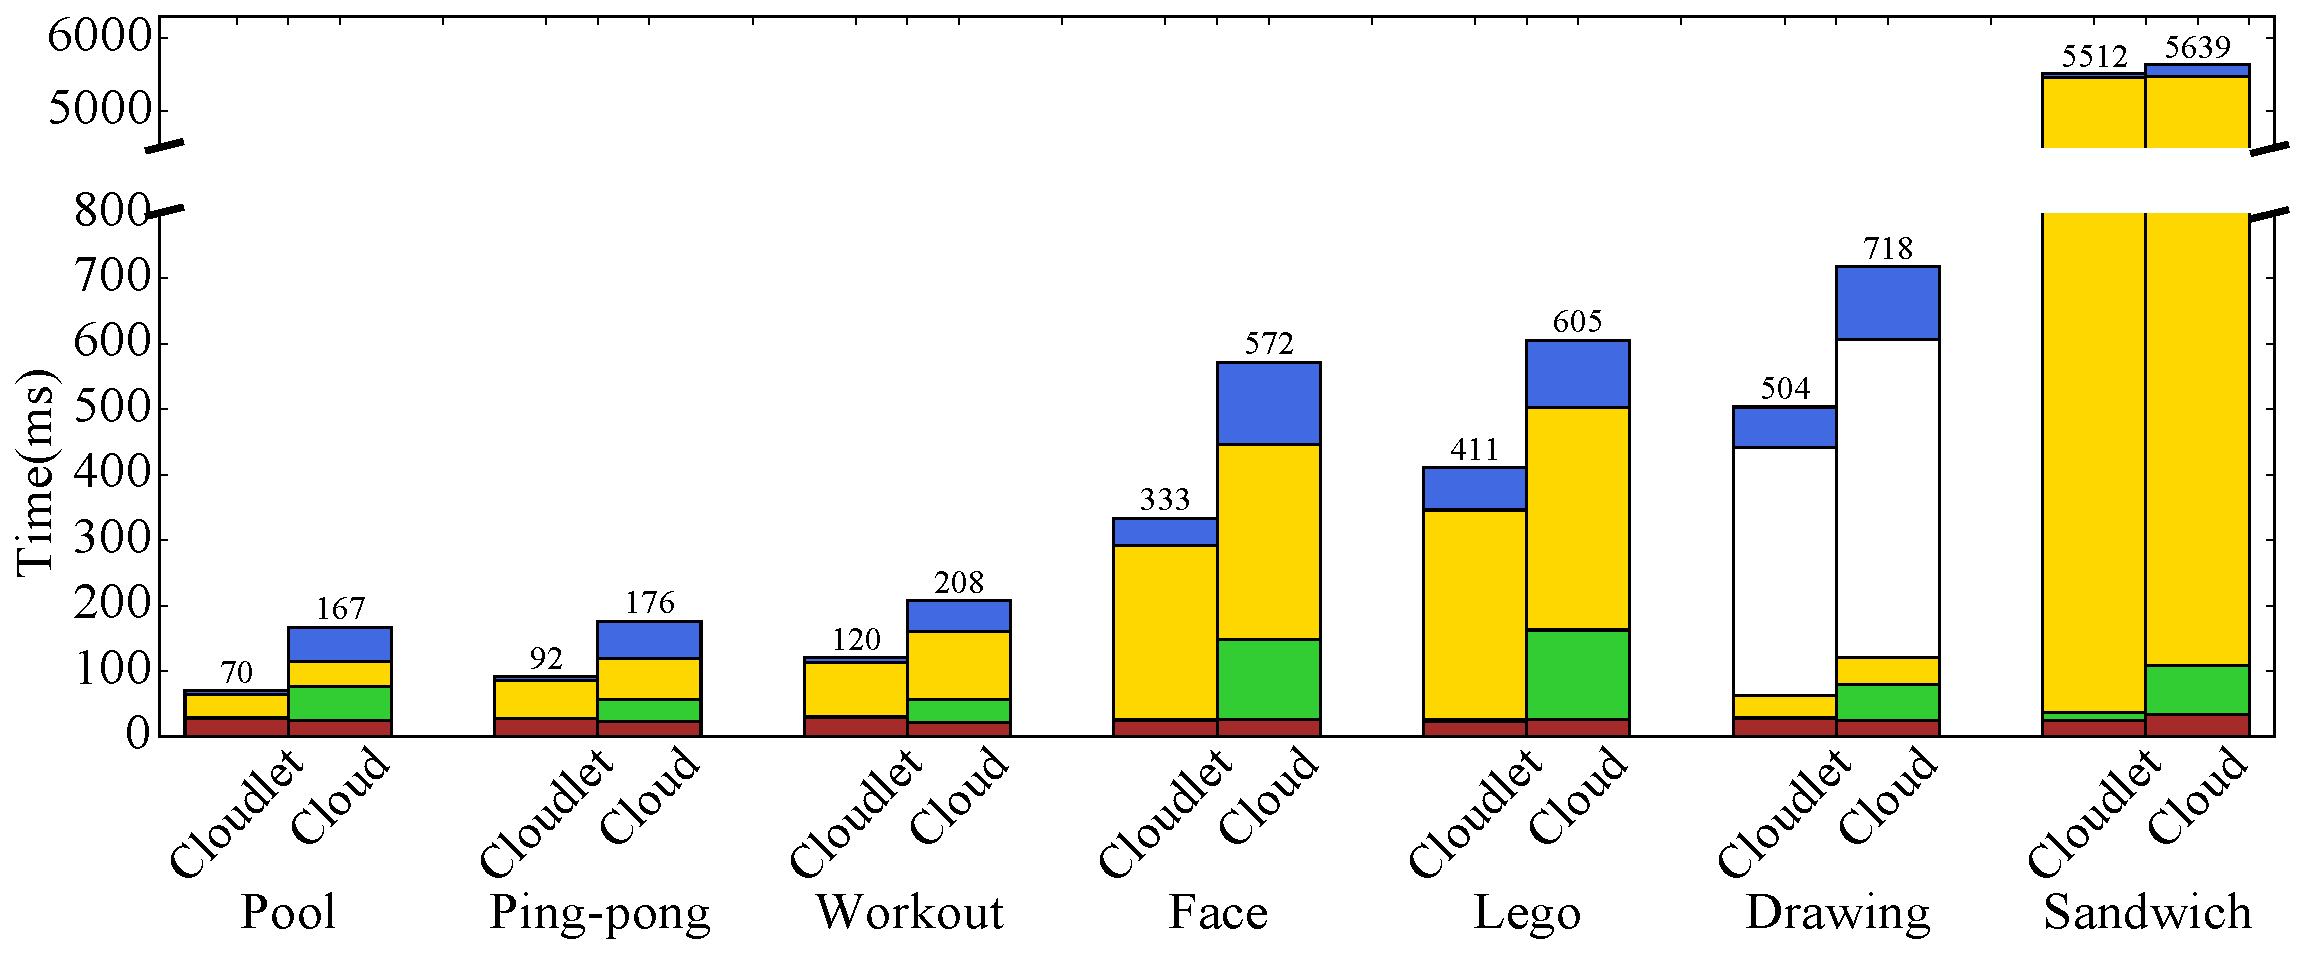
\includegraphics[height = 2in]{FIGS/pool-pingpong-workout-face-lego-draw-cooking-breakdown.pdf}
    \end{minipage}
    \hspace{-0.50in}
    \begin{minipage}{0.7in}
    \raisebox{0.5in}{
        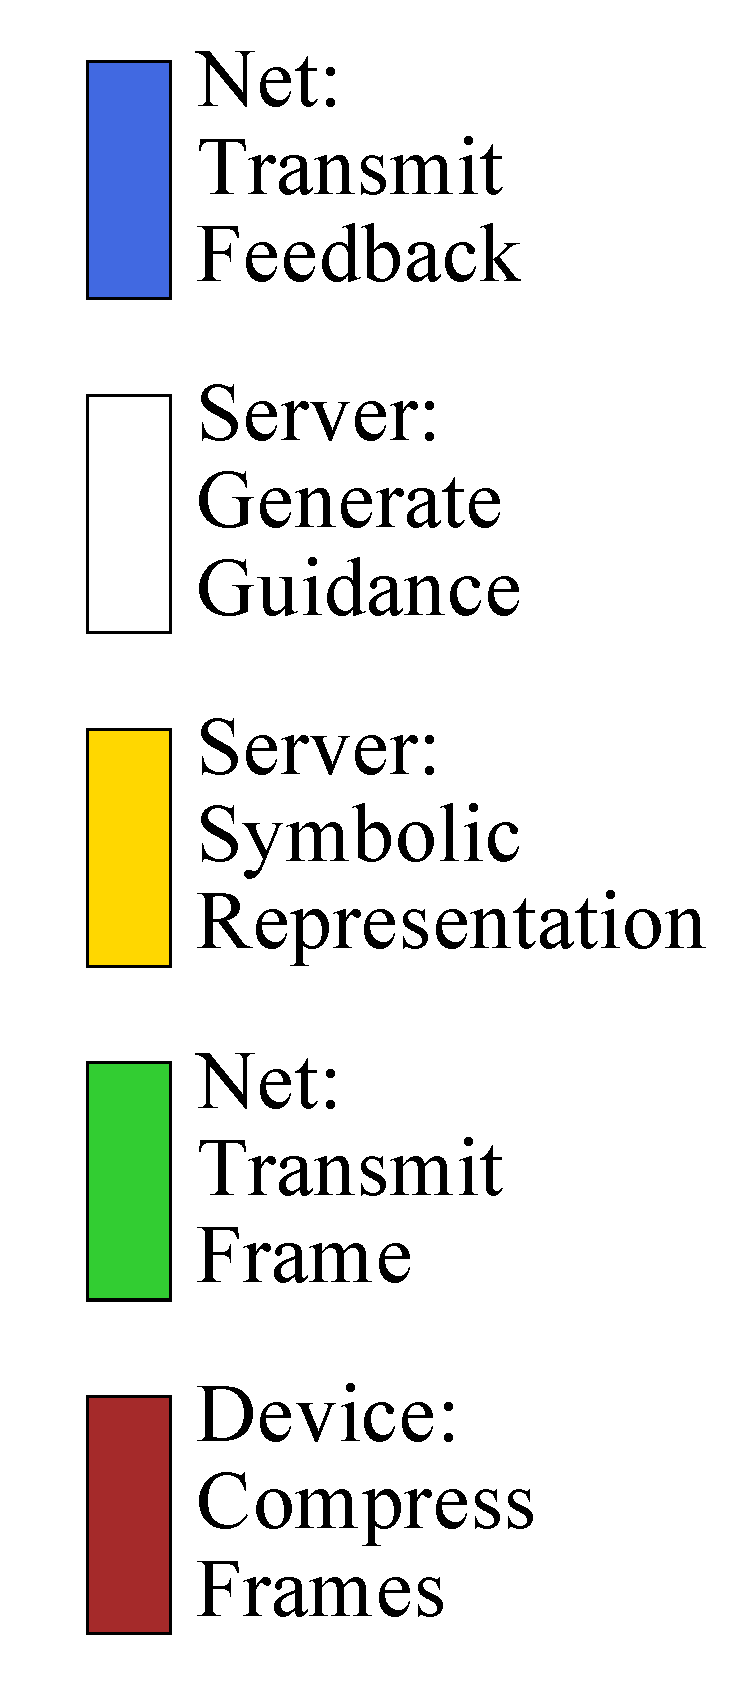
\includegraphics[height=1.9in]{FIGS/legend-breakdown.pdf}
    }
    \end{minipage}
    \vspace{-0.1in}
	\caption{Mean Latency Breakdown - Cloudlet vs. Cloud for Phone over WiFi}
    \vspace{-0.0in}
    \label{fig:breakdown}
\end{figure*}


Figure~\ref{fig:breakdown} shows the time breakdown of these assistants. For the
cloudlet case (left bars for each application), relatively little time is spent
on network transmission, which is the benefit of edge computing. When offloading
to the cloudlet, the server compute time consists of a significant portion, if
not the most significant part of the end-to-end latency. For applications
that use DNNs to process complex scenes, for example, Face and Sandwich, the
server computation time dominates.

\subsubsection{Wireless Network Characteristics}
The sensed data, e.g. images and videos from mobile devices, are transmitted to
a cloudlet through wireless communication. While IEEE 802.11 protocol is
widely-used at home and enterprise settings, the cellular network, particularly
LTE provides a better experience with its always-on ubiquitousness and large
area coverage. To this end, I will focus on LTE network as the primary wireless
communication protocol in the rest of my work.

LTE has unique characteristics in both latency and bandwidth. While previous
works~\cite{hu2016quantifying} and ~\cite{hadvzic2017edge} have experimentally
measured LTE's latency for mobile applications, the influence of LTE's bandwidth
and capacity on wearable cognitive assistance applications is mostly
unexplored.

The LTE uplink bandwidth is both limited and highly variant. LTE release 8 has a
theoretical a peak uplink data rate of 75 Mbps compared to 300 Mbps peak
downlink data rate. For LTE-Advanced, a major step toward 5G, the peak uplink
and downlink data rate are 1500 Mbps and 3000 Mbps respectively. In addition,
these theoretical peak data rates can only be achieved under idealized set-up
condition. For example, the LTE cell in test needs to be well isolated from
other cells while the test mobile device needs to be close to the base station.
Actual deployment has less bandwidth available~\cite{cox2012introduction}. For a
single user, the available bandwidth can be even less due to sharing. For
example, a 2012 study measured median LTE downlink and uplink bandwidth in US
commercial network to be 13 Mbps and 6 Mbps respectively~\cite{huang2012close}.
In 2017, the highest average upload bandwidth is 18 Mbps among providers in
US~\cite{PCMag2017}. In addition, LTE bandwidth has high
variance~\cite{winstein2013stochastic}. ~\cite{huang2012close} observed high
variation on LTE throughput not only for different users at different locations,
but also for the same user at the same location across different runs.

Gabriel applications put a high bandwidth demand on the network since they
continuously stream video data to cloudlets over wireless links. As a
comparison, Netflix recommends an internet connection speed of 5 Mbps to watch
its highly compressed HD video content. Gabriel applications would consume more
bandwidth due to on-the-fly compression. Hundreds of users simultaneously
streaming high-definition videos could easily saturate today's LTE uplink
capabilities~\cite{oyman2010toward}. Therefore, effective reduction of the
bandwidth consumption is essential to support concurrent running of many Gabriel
applications.

\subsection{Accelerators on Edge Nodes}
The computation capability of cloudlets, especially hardware accelerators, also
becomes a bottleneck with many users. The high demand for accelerator resources
comes from the widespread use of DNNs to solve computer vision tasks. DNNs'
superior learning ability enables them to advance the state-of-art accuracy. The
large capacity to learn comes from the sheer number of model parameters. For
example, the widely-used image classification network
ResNet-101~\cite{he2016deep} has more than 42 million parameters. Another
classifier network Inception ResNet V2 which achieves higher accuracy on
ImageNet~\cite{deng2009imagenet} has more than 53 million
parameters~\cite{huang2017speed}. For more sophisticated tasks, for example
object detection, additional layers are needed beyond image classifiers,
resulting in even more parameters. In addition, these networks are deep, with
tens to hundreds of layers in a sequence. Computational dependencies exist
among the bottom and top layers. The combined effect of a large number of both
parameters and layers is the high computational demands when using DNNs for
inference. In order to shorten computational latency, hardware accelerators that
can exploit parallel execution, for example GPUs, are commonly used for both
DNN training and inference. ASIC accelerators to further improve speed have also
been developed. For example, Google has deployed Tensor Processing Units (TPUs)
into their cloud to meet DNNs' computational
demands~\cite{jouppi2017datacenter}.

Despite many efforts in hardware design, the cost of DNN accelerators remains
high. For example, a Nvidia Pascal Titan X graphic card, a top-of-line GPU for
DNNs, costs around~\$1200~\cite{Nvidia2017TitanX}. Nevertheless, it can only run
the object detection network Faster-RCNN with ResNet101 at a speed of fewer than
10 frames per second (FPS)~\cite{huang2017speed}. Although large batch sizes
could theoretically improve the throughput, they often sacrifice application
latency and therefore are not suitable for many Gabriel applications. To support
more users with high demands on accelerators, Gabriel framework needs to
efficiently manage and share scarce and expensive acceleration resources among
concurrent users to reduce the cost of deployment.

\subsection{Difficulty of Development}

Gabriel applications are difficult to develop. Not only is the development
process slow, but specialized computer vision experience is also needed. It took
a researcher four months to build his first cognitive assistant for assembling
LEGO pieces~\cite{chen2018application}. The majority of time is spent on
learning the computer vision techniques and selecting robust algorithms to use
through trial and error. New developers would face the similar obstacles when
building these applications from scratch. As a result, the number of wearable
cognitive assistants available is quite limited. Therefore, Gabriel needs to be
extended with a toolchain to reduce the difficulty of development.

\begin{figure*}
  \centering
  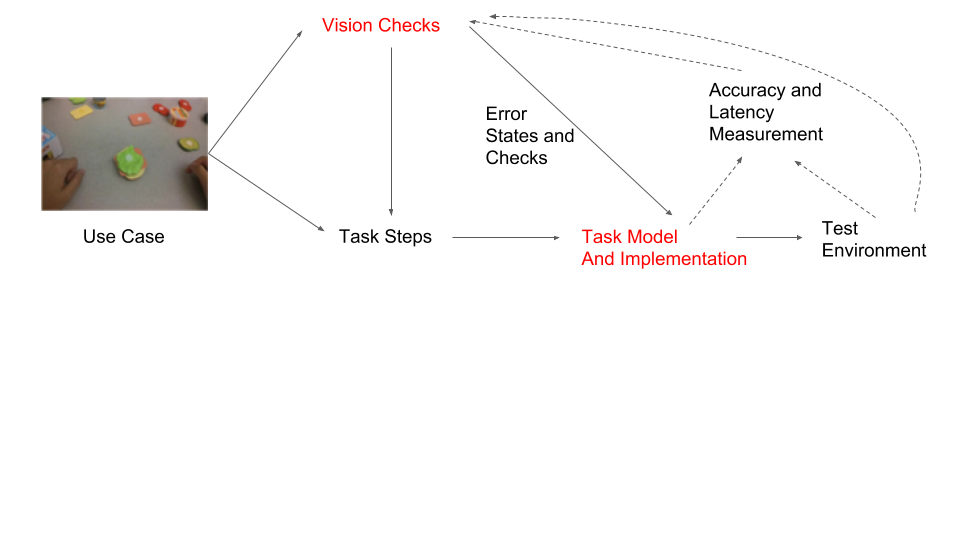
\includegraphics[trim={0 10cm 0 0},width=\linewidth]{FIGS/ad-hoc-workflow}
  \hspace{-0.50in}
	\caption{Development Workflow}
    \vspace{-0.0in}
    \label{fig:workflow}
\end{figure*}

The overall development workflow of wearable cognitive assistance is shown in
figure~\ref{fig:workflow}. After a use case is identified, developers would need
to identify meaningful visual states that can be detected using computer vision.
In the meantime, a task is divided into steps based on the use case and
detectable visual states. Task procedures could be changed to reduce the
difficulties of CV checks. In fact, since there is a human in the loop, relying
on humans to do what they are good at is the main reason that wearable cognitive
assistance can be implemented without solving perception and planning problems
intrinsic to robotics. Task procedures together with error states form a task
model. Developers implement the application according to the task model. After
 initial implementation, test runs and measurements are conducted to evaluate
the robustness of computer vision checks and end-to-end application latency.
This process is iterated until developers are satisfied.

Among all the development procedures, creating the computer vision checks to
detect user states consumes the most of development time and requires computer
vision expertise and experience. With the adoption of DNNs, developers no longer
need to spend days to select and tweak handcrafted features. Instead, the entire
model is trained end-to-end using labeled data. However, DNNs, with millions of
parameters to train, requires a significant amount of training data. Collecting
and labeling data are time-consuming and painstaking. Besides, to craft and
implement a DNN by hand is not trivial. Significant machine learning background
is needed to tweak network architectures and parameters. Therefore, developer
tools are needed to both help label the data and create deep neural networks.

In summary, implementing the workflow of cognitive assistance takes time and
efforts. Ad-hoc implementation requires a team of domain experts, developers and
computer vision experts. Such development model cannot scale to thousands of
applications. Therefore, Gabriel needs to be extended with tools to reduce the
effort of creating wearable cognitive assistants.

% \section{Bandwidth Reduction}

Gabriel applications continuously stream sensor data to the cloudlet. The richer
a sensing modality is, the more information can be extracted. Visual data from
cameras is one of such rich sensing modalities that wearable cognitive
assistance leverages. However, the last hop wireless bandwidth, especially LTE
bandwidth cannot support thousands of users simultaneously streaming high
definition videos. Therefore, to effectively scale wearable cognitive
assistance, we need to reduce the bandwidth consumed. There are three techniques
I will explore to reduce the bandwidth cost by exploiting the unique properties
of the workload. We have shown the effectiveness of these techniques with drone
footages. Further experiments with first-person videos will be done to show
their effectiveness for wearable cognitive assistance.

\subsection{Early Discard}
Early discard refers to the technique that filters and discards contents in
early stages of computation. An example system that uses early discard is an
unindexed search system~\cite{satyanarayanan2010searching}. In the mobile
computing context, ~\cite{hu2015case} explored using image-level simple computer
vision algorithms, for example blur and color detection, to suppress
transmission of uninteresting video frames.

In Gabriel applications, an efficient early discard system that filters out
uninteresting frames before transmission can reduce the bandwidth consumption.
For example, in the Lego assistant, all the assembled Lego pieces are placed on
a Lego board with black boundaries. Some frames do not contain the Lego board
due to user movement. Without further analysis, the application knows these
frames do not contain useful information since the board is not present. If an
efficient contour detection of black boundaries can be performed on the wearable
device, the application can save the unnecessary bandwidth consumed to transmit
the uninteresting frames.

There exists a tradeoff between computation and network transmission for early
discard. To one end, if the wearable device is powerful enough to perform all
the computation on-device within latency constraints, the bandwidth cost would
be minimal because there is no need to offload the computation. To the other
extreme, if the wearable device is very weak, all the sensor data then needs to
be shipped to the cloudlets for processing. In fact, image compression can be
thought as an early discard technique at the pixel level. It uses the
computation onboard to remove the duplicate data sent over the network.

To explore the effectiveness of early discard, we conducted experiments in a
small drone setting. Drones typically can carry more computational power than
wearable devices. Therefore they can be thought of futuristic wearable devices
with large computation capability. In my thesis, I will run similar experiments
on wearable devices with first-person videos. Below we will present our
experiments on drone videos to demonstrate the effectiveness of early discard.

\begin{figure*}
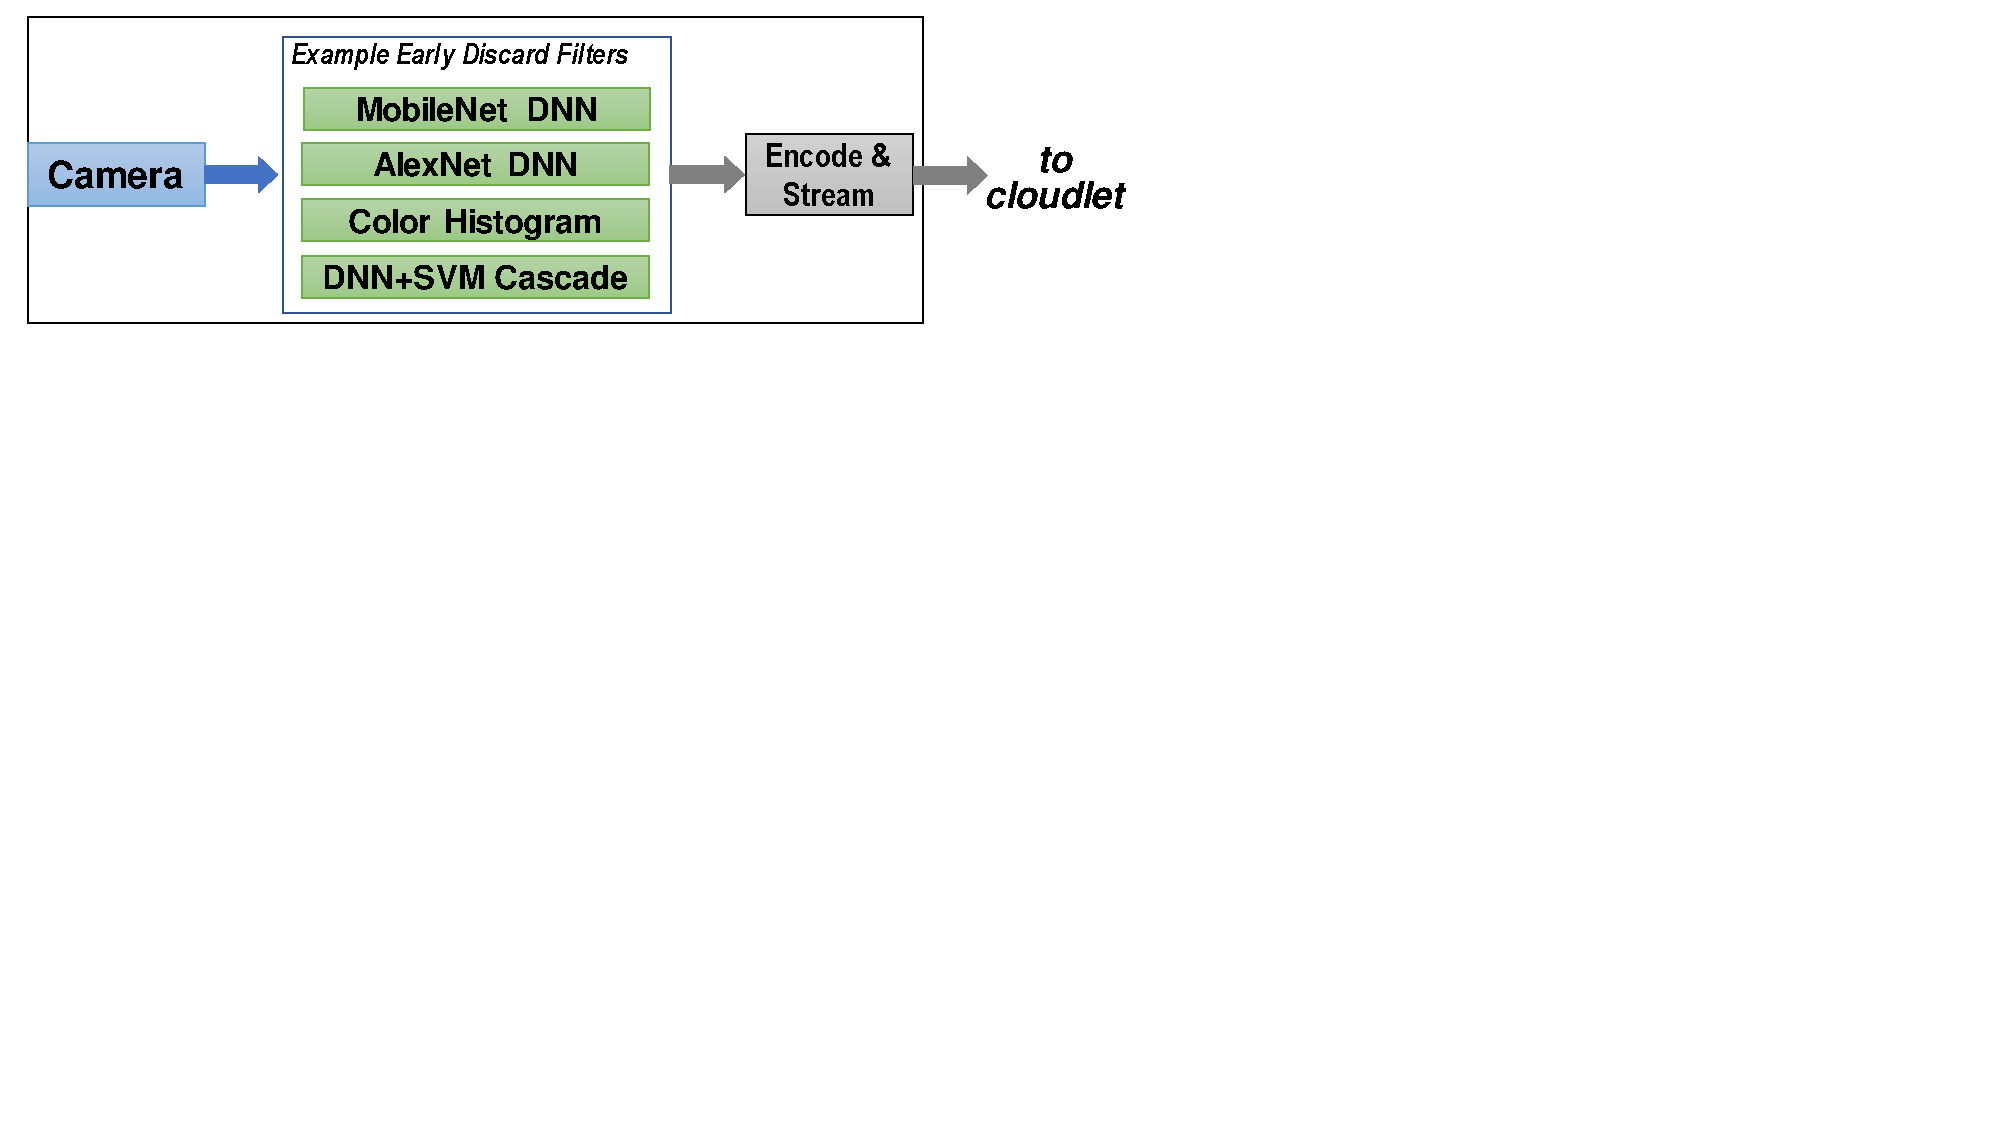
\includegraphics[scale=0.8,trim={0 13.5cm 10cm 0},clip]{FIGS/fig-early-discard.pdf}\\
\caption{Early Discard Pipeline.}
\label{fig:ondrone}
\vspace{-0.2in}
\end{figure*}


As shown in Figure~\ref{fig:ondrone}, we envision a choice of weak detectors
being available as early discard filters on a drone, with the specific choice of
filter being mission-specific. We use image classification as early discard
filters on the drone: it is not necessary to know exactly where in the frame a
relevant object occurs. This suggests that MobileNet would be a good choice as a
weak detector. Its speed of 352 ms per frame on Nexus 6 yields less than 3 fps.
However, its speed of 13 ms per frame on Jetson yields more than 75 fps. If
Jetson-class hardware was to be available on future smartphones, MobileNet
would be usable at a full frame rate. We therefore use MobileNet on the drone for
early discard in our experiments.

\begin{figure*}
\centering
\begin{tabular}{|p{1cm}|p{2cm}|p{2cm}|p{2.5cm}|p{2cm}|p{3cm}|}
\hline
   & Detection & Data & Data & Training & Testing \\ 
Task& Goal & Source & Attributes & Subset & Subset\\ 
\hline
T1 & {\small People in scenes of daily life}&{\small Okutama Action Dataset~\cite{Barekatain2017}}&\makecell[tl]{\small 33 videos \\\small 59842 fr\\\small 4K@30~fps}&\makecell[tl]{\small 9 videos\\\small 17763 fr}&\makecell[tl]{\small 6 videos\\\small 20751 frames}\\ 
\hline
T2 &{\small Moving cars}&{\small Stanford Drone Dataset~\cite{Robicquet2016}}&\makecell[tl]{\small 60 videos \\\small 522497 fr\\\small 1080p@30~fps}&\makecell[tl]{\small 16 videos\\\small 179992 fr} & \multirow{4}{*}{\parbox{3cm}{\centering\small 14 videos 92378 fr\\ Combination of videos from each dataset. T1's test uses a subset that do not have unlabeled human.}} \\ \cline{1-5}
T3 &{\small Raft in flooding scene}&{\small YouTube collection~\cite{YouTube1}}&\makecell[tl]{\small 11 videos \\\small 54395 fr\\\small 720p@25~fps}&\makecell[tl]{\small 8 videos\\\small 43017 fr} & \\ \cline{1-5}
T4 &{\small Elephants in natural habitat}&{\small YouTube collection~\cite{YouTube2}}&\makecell[tl]{\small 11 videos \\\small 54203 fr\\\small 720p@25~fps}&\makecell[tl]{\small 8 videos\\\small 39466 fr} & \\ \cline{1-5}
\hline
\end{tabular}
\vspace{0.2in}
\begin{captiontext}
fr = ``frames''\\
fps = ``frames per second''\\
No overlap between training and testing subsets of data
\end{captiontext}
\caption{Benchmark Suite of Video Traces}
\label{fig:benchmarksuite}
\end{figure*}

Our experiments on the {\xc EarlyDiscard} strategy used benchmark tasks suite
described in figure ~\ref{fig:benchmarksuite}. We used Nvidia Jetson TX2 as the
drone platform. We use both frame-based and event-based metrics to evaluate the
MobileNet filters. These experiments demonstrate that significant bandwidth
saving can be achieved while maintaining final detection accuracy through
interesting frames selection with filters running on the mobile device.

\begin{figure}
    \centering
    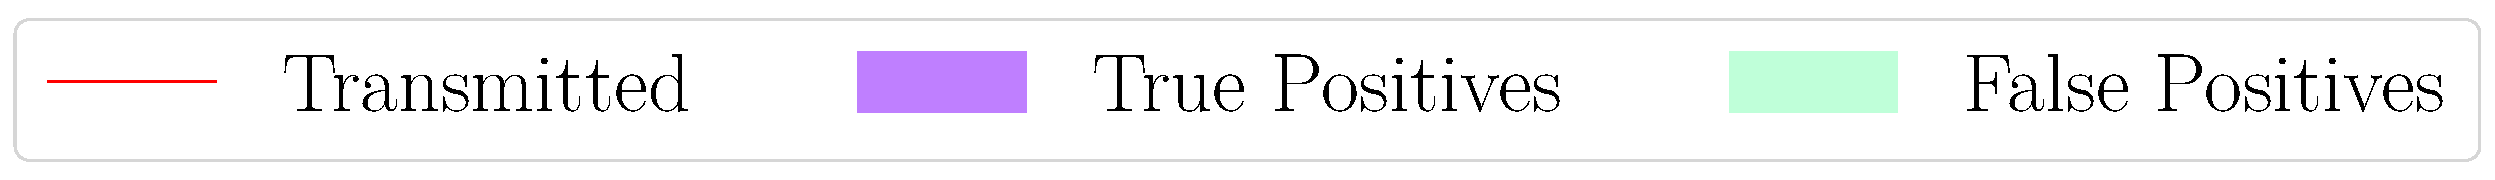
\includegraphics[width=0.9\linewidth]{FIGS/fig-event-recall-frame-percentage-legend.pdf}
    \hspace*{-0.35in}
    \begin{subfigure}[T1]{
        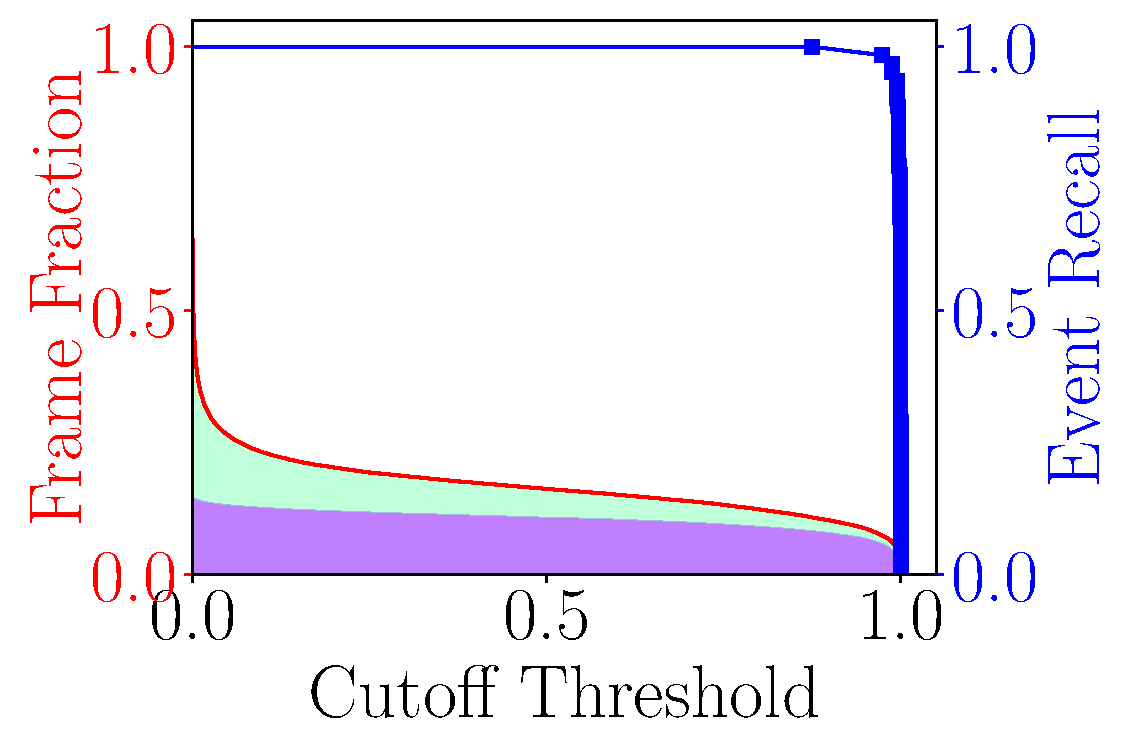
\includegraphics[width=0.4\linewidth]{FIGS/fig-event-recall-frame-percentage-vs-threshold-okutama.pdf}}        
    \end{subfigure}
    \begin{subfigure}[T2]{
      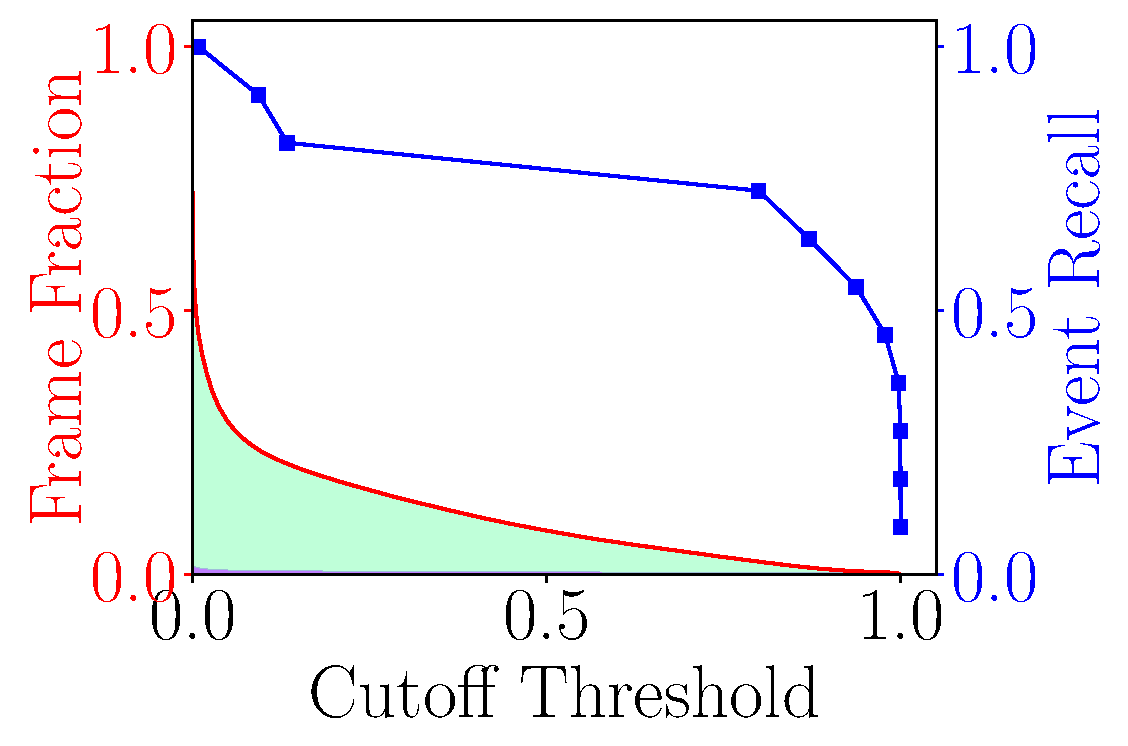
\includegraphics[width=0.4\linewidth]{FIGS/fig-event-recall-frame-percentage-vs-threshold-stanford.pdf}}
    \end{subfigure}
    \hspace*{-0.35in}    
    \begin{subfigure}[T3]{
      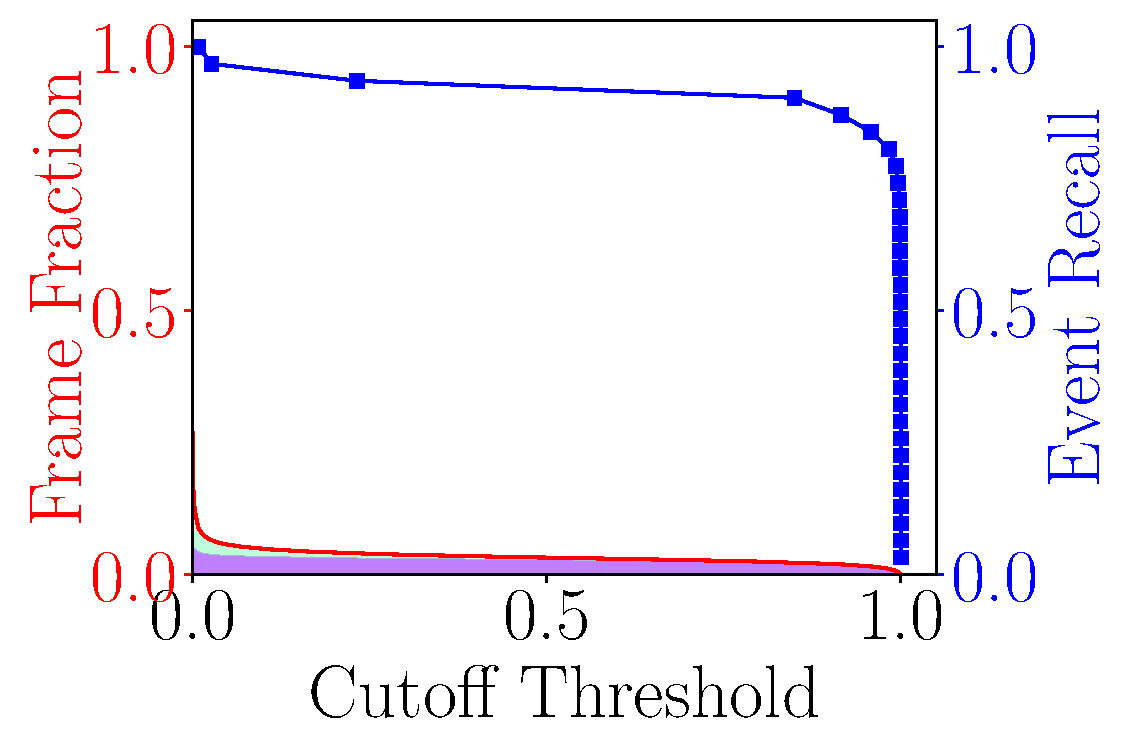
\includegraphics[width=0.4\linewidth]{FIGS/fig-event-recall-frame-percentage-vs-threshold-raft.pdf}}
    \end{subfigure}
    \begin{subfigure}[T4]{
      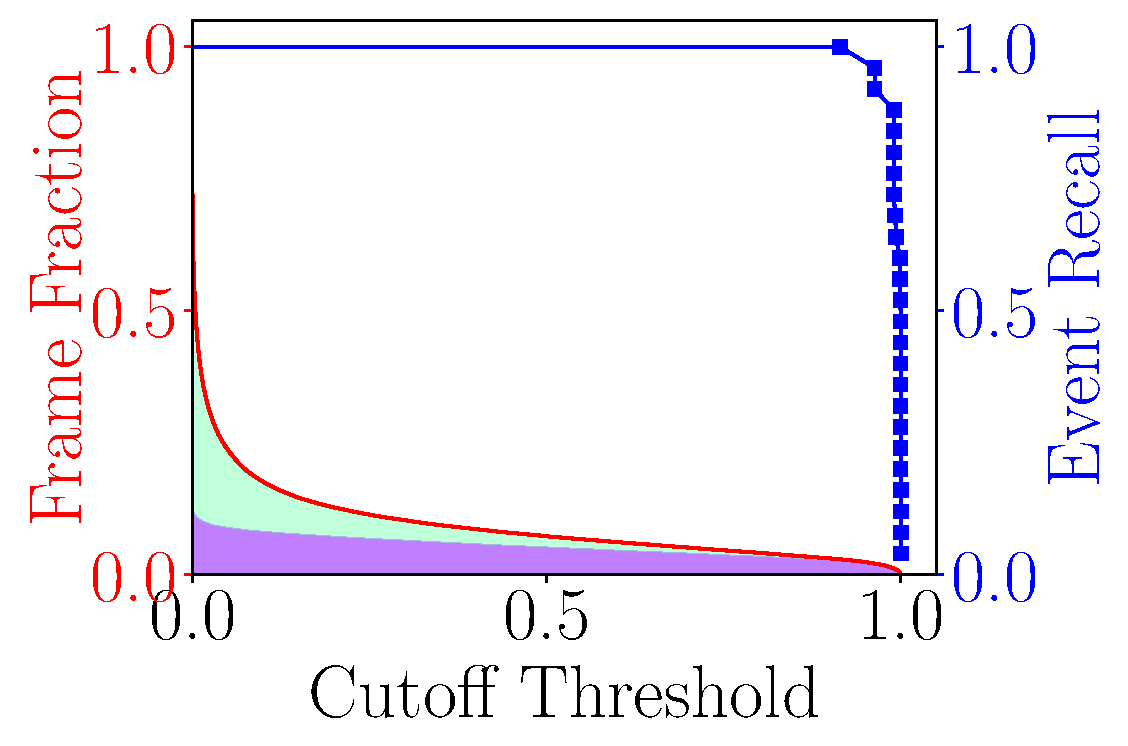
\includegraphics[width=0.4\linewidth]{FIGS/fig-event-recall-frame-percentage-vs-threshold-elephant.pdf}}
    \end{subfigure}
\vspace{-0.2in}
\caption{Where the Bandwidth Goes}
\label{fig:earlydiscard-frame-percent-breakdown}
\end{figure}

\noindent{\textbf{Drone Filter Accuracy}}: The output of a drone filter is the
probability of the current tile being ``interesting.''  A tunable {\em cutoff
  threshold} parameter specifies how interesting is ``interesting enough'' for
transmission to the cloudlet.  All tiles, whether deemed interesting or not,
are still stored in drone storage for post-mission processing.

Events (such as detection of a raft in T3) occur in consecutive frames, all of
which contain the object of interest. A correct detection of an event is
defined as at least one of the consecutive frames being transmitted to the
cloudlet.  Blue lines in Figure~\ref{fig:earlydiscard-frame-percent-breakdown}
shows how the event recalls of drone filters for different tasks change as a
function of cutoff threshold. As the figure shows, the MobileNet DNN filter is
able to detect all the events for T1 and T4 at a high cutoff threshold. For T2
and T3, the majority of the events are detected. Achieving high recall on T2
and T3 (on the order of 0.95 or better) requires setting a low cutoff
threshold.  This leads to the possibility that many of the transmitted frames
are actually uninteresting (i.e., false positives).

\noindent{\textbf{False negatives}}: As discussed earlier, false negatives are
a source of concern with early discard.  Once the drone drops a frame
containing an important event, improved cloudlet processing cannot help. The
results in the third column of Figure~\ref{fig:early-discard-results} confirm
that there are no false negatives for T1 and T4 at a cutoff threshold of 0.5.
For T2 and T3, lower cutoff thresholds are needed to achieve perfect recalls.

\begin{figure}
\centering
\begin{tabular}{|c|c|c|c|c|c|c|}
\hline
   &        &Dete-       &Avg&Total&Avg&Peak\\
   &Total&cted&Delay&Data&B/W&B/W\\
   &Events&Events&(s)&(MB)&(Mbps)&(Mbps)\\ 

\hline
\small
T1 & \phantom{0}62  & 100~\%       &  \phantom{0}0.1&\phantom{0}441  &  5.10     &   10.7  \\
\hline
T2 & \phantom{0}11  & \phantom{0}73~\%      & \phantom{0}4.9 & \phantom{00}13            &  0.03 & \phantom{0}7.0 \\ % 100% recall at 47% of frames, 82% recall at 21% of frames
\hline
T3 & \phantom{0}31  & \phantom{0}90~\%  & 12.7 & \phantom{00}93  &  0.24 &  \phantom{0}7.0 \\ % 100% recall at 9% frames
\hline
T4 & \phantom{0}25  & 100~\%       & \phantom{0}0.3 & \phantom{0}167  &  0.43 &  \phantom{0}7.0 \\
\hline
\end{tabular}\\
\caption{Recall, Event Latency and Bandwidth at Cutoff Threshold 0.5}
\label{fig:early-discard-results}
\end{figure}

\noindent{\textbf{Result latency}}: The contribution of early discard processing
to total result latency is calculated as the average time difference between the
first frame in which an object occurs (i.e., first occurrence in ground truth)
and the first frame containing the object that is transmitted to the backend
(i.e., first detection). The results in the fourth column of
Figure~\ref{fig:early-discard-results} confirm that early discard contributes
little to result latency. The amounts range from 0.1~s for T1 to 12.7~s for T3.
At the times cale of human actions such as dispatching of a rescue team, these
are negligible delays.

Although the general approach of early discard would apply for wearable
cognitive assistance, how to apply this technique to wearable devices still
needs investigation. First, wearable devices in general have even less
general-purpose computation capabilities. Due to the small form factor and heat
dissipation constraints, the mobile CPUs in wearable devices are optimized for
power instead of performance. In fact, many smart glasses today rely on a user's
smartphone to process information. For instance, one of Google Glasses' main use
cases when it was first released is to display notifications from smartphone
applications, such as CNN and EverNote~\cite{theverge2013}. Second, there is a
strong trend to put hardware DNN accelerators into embedded devices to perform
some analysis of visual data. There are many efforts from both industry and
academia. For example, Microsoft HoloLens has a special Holograhic Processing
Unit~\cite{theregister2016} to map the environment in 3D. Recently released
Google Pixel 2 smartphone have visual cores built-in for future-proofing although
not all of them are being actively used now~\cite{androidcentral2017}. In
academia, there are strong interests in DNN compression and optimization for
embedded devices so that the inference can run natively on
device~\cite{han2015deep}~\cite{han2016eie}. Therefore, it is likely that smart
glasses' computation capabilities, especially their capabilities of executing
DNNs, would vary greatly.

I would like to further explore how to create filters for a variety of
heterogeneous smart glasses with or without accelerators in my thesis. I plan to
formulate the problem as an optimization problem that optimizes for the least
amount of bandwidth consumption constraint by the application latency requirement.
To its simplistic form, the problem can be written as
\begin{equation*}
\begin{aligned}
& \text{minimize} & & AverageDataTransmittedPerImage \\
& \text{subject to} 
  & & OnBoard Processing Time \\
  & & & + Network Transmission Time \\
  & & & + Server Computation Time \leq Application Latency Requirement 
\end{aligned}
\end{equation*}
I also plan to design tools that will generate filters given these constraints.

\subsection{Just-in-time Learning}
Just-in-time-learning (JITL) refers to the technique that tunes the processing
pipeline to the characteristics of the current scenario in order to reduce
transmitted false positives from the client, therefore reduce wasted bandwidth.
When training DNNs to recognize and detect objects, machine learning experts do
their best to obtain training examples from the same distribution of the test
data. In other words, best efforts are made to acquire training examples from
environments similar to test environment in terms of lighting, occlusion, and
many other aspects. However, as a Gabriel application could be used in any
environment, it is not realistic to assume all of them can be truthfully
represented by the training data. For test environment that does not look
similar to the training environment, the detection accuracy could be lower.
Just-in-time-learning aims to alleviate the generalization problem by making
each test environment represented in the training samples. Such goal can be
achieved by quick collecting a small number of examples drawn from the actual
test environment and iteratively training an existing model with the newly
collected data in a short time.

I plan to focus on mechanical assembly tasks when applying just-in-time learning
to wearable cognitive assistance. For mechanical assembly tasks, the environment
a user is in usually does not change significantly. For example, a user might
sit in front of a desk for most of the time. The relatively stable environment gives
us opportunities to leverage the human in the loop to provide false positive
examples. Before the application starts, a cognitive assistant could ask the
user to look around her environment with the assembly kits put away for a short
period of time. By construction, any positive predictions are false positives.
They are excellent negative training examples because they are taken in the
actual test environment. I plan to explore multiple methods to make use of these
newly collected data. First, feature matching could be used to identify
subsequent false positives. Specifically, a false positive feature pool can be
built for the particular test environment with the newly collected negative
data. For each prediction at application runtime, a matching is performed to see
if it is close enough to items in the false positive feature pool. Second,
researchers have shown positive results from train image segmentation DNNs with
a small number of examples for a few iterations to fit the model better to the
test environment. I plan to explore similar techniques in object detections.

\subsection{Context-awareness}

The essence of this approach is to leverage unique attributes of the current
task to improve the speed and accuracy of image processing on the mobile device.
By definition, this approach is ad hoc in character. However, the wins can be
significant. Consider the fuchsia colored screw in RibLoc cognitive assistant as
an example. Since the color of the screw is rarely seen in everyday objects,
cheap color filtering instead of DNNs can be used to filter interesting frames.

%% searching for survivors in the
%% ocean after a shipwreck.  Suppose the standard approach for detecting
%% survivors in search and rescue missions involves detection of human
%% faces and bodies~(similar to T1), or distinctive actions such as
%% waving.  These are used as the basis of early discard
%% at the beginning of the mission.  During the mission, as personnel
%% review results that are presented to them after cloudlet processing,
%% they notice that all survivors are wearing flotation devices
%% (lifejackets) that have a distinctive color.  Against the
%% blue-green background of the ocean, detecting this color is a fast,
%% accurate, and computationally cheap way of detecting survivors.
%% Figure~\ref{fig:shipwreck}(a) gives an example of such a scene.
%% However this optimization is unique to this mission.  On a different
%% mission that also involves a shipwreck, the lifejackets may be of a
%% different color.  Or, because of the late afternoon timing of the
%% mission and the consequent low angle of the sun, too many false
%% positives may arise from reflections off the water if reddish-orange colors
%% are used as the basis of early discard.

%% \begin{figure}
%% \centering
%% 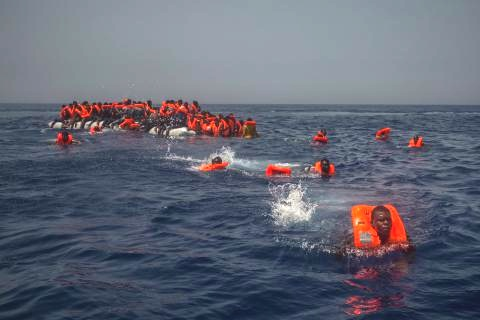
\includegraphics[width=2.5in]{FIGS/fig-shipwreck6.jpg}\\
%% (a) Motivating Image\\[0.2in]
%% \caption{Example of Context-Aware Strategy}
%% \label{fig:shipwreck}
%% \vspace{-0.2in}
%% \end{figure}


%% By the classic metrics of machine learning, the use of such heuristics
%% is viewed as ``overfitting'' and therefore something to be avoided at
%% all costs.  Yet, in practical terms and in the narrow context of this
%% mission, the heuristic offers many advantages without compromising
%% accuracy.  On some missions, the heuristic may even prove to be more
%% accurate than a DNN.  We consider it important to allow mission
%% personnel to take advantage of such context-aware optimizations.

%% Mission personnel can specify parameters to early filters by example. This can
%% done by drawing bounding boxes around the relevant parts of images that were
%% presented after cloudlet processing. Filters can be selectively activated or
%% deactivated, and combined to generate complex search predicates. They can be
%% used on the drone both for early discard of future video, as well as
%% re-examination of stored video. When the accuracy of the uploaded filter is
%% better than that of the default DNN filter, a re-examination of stored video can
%% yield hits that were missed earlier. These new hits can be downloaded to the
%% cloudlet for further processing. The context-aware filter is thus being used
%% both for reachback from already-captured video, as well as for early discard on
%% future video.

To demonstrate the effectiveness of this strategy, we apply it in the drone
context using a simple color filter in T3. In each raft search video, we
randomly pick a frame that contains a raft (true positive), and obtain the color
of the most distinctive region of the raft. Using the hue, saturation, and value
(HSV) color space attributes of this region, we apply a color filter to all the
other frames of the video. If a significantly large area of a frame passes this
filter, the frame is marked as positive. Otherwise, it is marked as negative.

\begin{figure}
\centering

\begin{tabular}{|l|l|l|l|}
\hline
        & \begin{tabular}[c]{@{}l@{}}Precision using\\ DNN (\%)\end{tabular} & \begin{tabular}[c]{@{}l@{}}Precision using\\ color filter (\%)\end{tabular} & \begin{tabular}[c]{@{}l@{}}Recall\\ (\%)\end{tabular} \\ \hline
Video 1 & 92.4                                                               & 95.3                                                                        & 89.1                                                  \\ \hline
Video 2 & 51.9                                                               & 76.1                                                                        & 90.0                                                  \\ \hline
Video 3 & 41.3                                                               & 84.3                                                                        & 88.6                                                  \\ \hline
\end{tabular}\\[0.1in]

(a) Accuracy\\[0.1in]

\begin{tabular}{|l|l|l|l|l|l|l|}
\hline
\multirow{2}{*}{} & \multicolumn{2}{c|}{Jetson} & \multicolumn{2}{c|}{Joule}   & \multicolumn{2}{c|}{Nexus 6}   \\ \cline{2-7}
                  & DNN                 & Color & DNN                  & Color & DNN                  & Color \\ \hline
Video 1           & \multirow{3}{*}{13} & 6.2   & \multirow{3}{*}{37} & 9.8   & \multirow{3}{*}{352} & 27.5  \\ \cline{1-1} \cline{3-3} \cline{5-5} \cline{7-7}
Video 2           &                     & 6.3   &                      & 9.7   &                      & 26.3  \\ \cline{1-1} \cline{3-3} \cline{5-5} \cline{7-7}
Video 3           &                     & 9.5   &                      & 12.3  &                      & 36.1  \\ \hline
\end{tabular}\\[0.1in]

(b) Processing time (ms)\\
\caption{Detection Results on T3 Using Color Filters}
\label{fig:colorfilter-results}
\vspace{-0.2in}
\end{figure}

Figure~\ref{fig:colorfilter-results} shows the results of using this
approach on three representative videos in T3.  Keeping recall fixed
at a high value (fourth column of
Figure~\ref{fig:colorfilter-results}(a)), the second and third columns
show the precision achieved using a DNN and a color filter.  For all
three videos, the precision using a color filter is better than the
precision using a DNN.  The difference is modest for Video 1, but
considerable for Video 2 and Video 3.  In other words, the context
aware approach is consistently more accurate.  This improvement in
accuracy does not come at a sacrifice in speed.  On the contrary,
Figure~\ref{fig:colorfilter-results}(b) shows that the DNN on the
Jetson takes 2--3 times the processing time of the color filter.  On
the Joule and the Nexus 6, it takes 8--10 times.  These results show
the high value of using context-aware knowledge.  What the DNN
provides is generality, combined with reasonable accuracy.  At the
beginning of a mission, when little is known about the
context-specific search attributes of the target, the DNN is the only
choice.  As the mission progresses, the early results may hint at the
attributes of a highly effective and cheap context-aware filter.

Although Gabriel applications do not have a human in the loop to specify filter
parameters, context-awareness can still be applied to wearable cognitive
assistance. In fact it could serve both as a mean to reduce bandwidth
consumption and as a method to reduce server computation latency. To achieve the
former goal, we can generate a suite of early-discard filters at training time
using different algorithms. When the application first starts, we can ask the
user to look around her environment and show us a few objects that will be used.
All early-discard filters can be evaluated during this ``warm-up'' time by
checking how many false positives and false negatives they produce. A filter
that performs the best in this test environment will be selected for application
usage. To be able to achieve such context-awareness, many challenges exist,
e.g. what metrics to use to evaluate these early discard filters, how to quickly
identify the best one to use, where should the computation happen, and how to
efficiently transmit context-aware updates to the client. I plan to explore
these questions in my thesis. In addition, such dynamic selection of CV
algorithms can be applied for processing at the edge nodes as well. We could
build upon the multi-algorithm acceleration approach described
by~\cite{chen2017empirical} to dynamically select a cheap algorithm to use from
auto-generated models in order to reduce processing latency.

% \section{Gabriel Deployment System}

Previous research on wearable cognitive assistance~\cite{chen2017empirical} has
focused on meeting application latency requirements and assumed abundant
resources on the cloudlets. However, when there are many users in the system
and the utilizations of system resources are high, both the compute and the
memory at the cloudlets can become scarce. Reduction of the application
footprint on cloudlets is needed in order to scale better.

\begin{figure}[h]
  \centering
  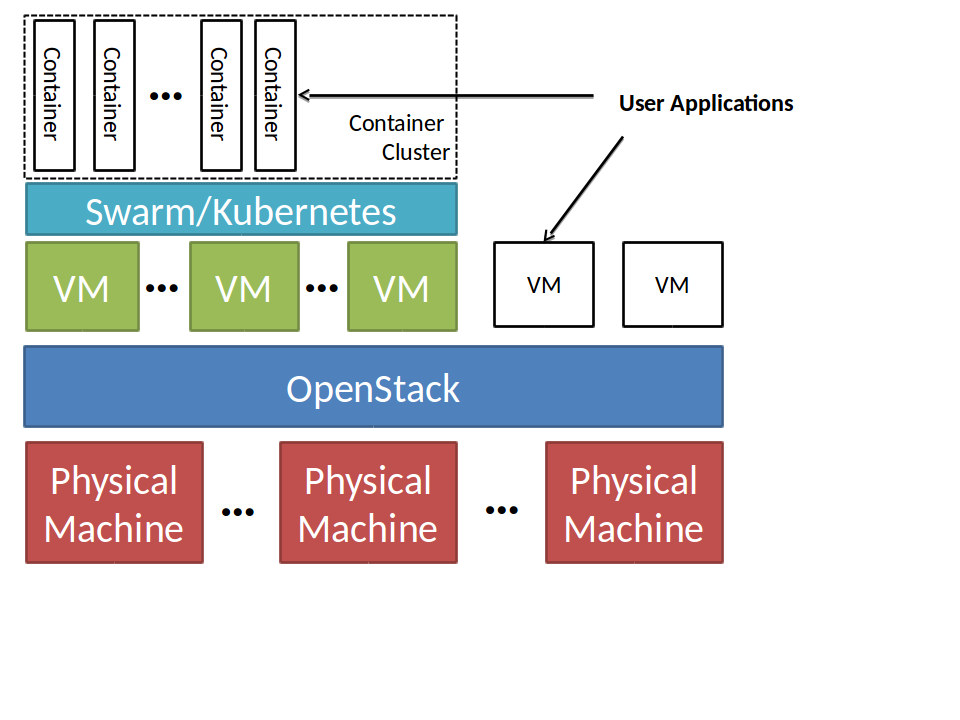
\includegraphics[trim={0 1.5in 0 0},clip,width=5in]{FIGS/cloudlet-gateway}
  \caption{Container and Virtual Machine Virtualization on Cloudlets}
  \label{fig:cloudlet-gateway}
  \end{figure}

Virtual machines (VMs) have been used to provide isolation among edge node
tenants~\cite{ha2014towards}. While VMs virtualize at the hardware level and
provide strong isolation among tenants, they also have a large footprint since
each virtual machine has its own kernel. In the meantime, some applications do
not need the strong isolation provided by VMs. For example, applications
published by the same developer or company would have stronger trusts about the
integrity of the software. Therefore, for these applications, using more
lightweight virtualization constructs, for instance, containers, can help reduce
the application footprint on cloudlets.

Figure~\ref{fig:cloudlet-gateway} shows an edge node implementation that
combines lightweight container virtualization with strongly isolated virtual
machines. It adopts a Container-on-top-of-VM approach. Application providers on
the cloudlets can create container clusters for managing multiple applications
or instances of an application using the lightweight containers. In the
meantime, different providers are isolated by VMs for better control. The edge
node deployment system also supports applications to use a combination of
virtual machines and containers. For example, an application might have some
components in Windows VMs while other components run inside Linux containers.
When this combination of virtualization is used, the system provides a DNS
service to help resolve hostnames.

\begin{figure}[h]
  \centering
  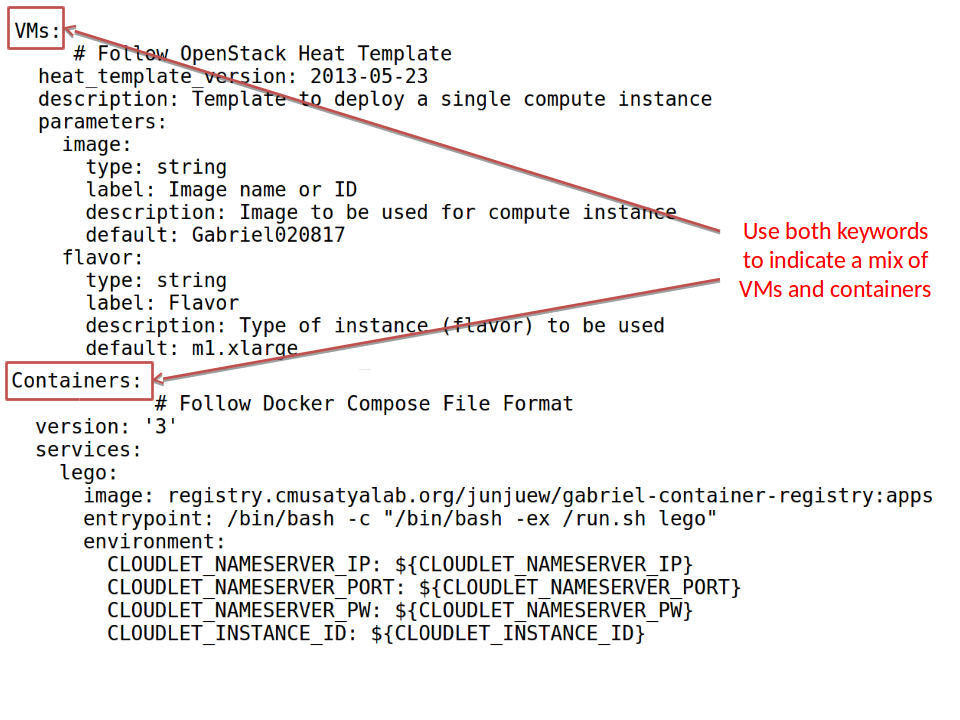
\includegraphics[trim={0 1.5in 0 0},clip,width=5in]{FIGS/cloudlet-app-configuration}
  \caption{Application Deployment Template with Virtualization Type Specified}
  \label{fig:cloudlet-app-configuration}
  \end{figure}


In order to specify virtualization techniques to use, developers only need to
modify their existing orchestration templates to include their choice of
virtualization. The system's annotation uses YAML~\cite{ben2005yaml} and follows
the convention of orchestration frameworks, including OpenStack Heat and Docker
Swarm. Figure~\ref{fig:cloudlet-app-configuration} shows an application
configuration file that adopts a mixed of virtual machine and container
virtualization. Components with different virtualization are separated into
different sections. Developers mark each section with the virtualization
technique they want to use. Specifications inside each section correspond to the
template consumed by the underlying orchestration frameworks.

% \section{Gabriel Acceleration Framework}

DNNs have been widely adopted as the de facto algorithms to use for analyzing
the image and video data. Therefore, running DNNs to analyze images is a common, if
not the most common, workload Gabriel needs to support. Due to the parallel
nature of DNN computation, such workload can be accelerated by special
hardware, including GPUs, FPGAs, and custom ASICs.

On cloudlets, due to physical constraints and economic decisions, we are
likely to see a wide range of heterogeneous accelerators. Some edge deployment
may have a cluster of custom ASIC DNN accelerators with proprietary drivers.
Others might use commodity GPUs. Some may not have any accelerators at all. Such
heterogeneity of acceleration capabilities has a direct impact on application
latencies and the number of users an edge node can serve. While hardware
capabilities vary, applications' needs on acceleration resources vary as well.
Applications may use DNNs of different sizes based on the complexity of their
task. For example, the Face Recognition Assistant developed uses a much smaller
network than the Sandwich Assistant in~\cite{chen2017empirical}. As a result,
the Face Assistant does not need a GPU to meet its latency requirement while
the Sandwich Assistant does.

Given the heterogeneity in both hardware capabilities and application demands, I
plan to study how to effectively federate cloudlets with different accelerators
to better serve applications with different needs. The heterogeneity can be both
inter-cloudlet and intra-cloudlet. I plan to address inter-cloudlet
heterogeneity from a cloudlet discovery perspective. Specifically, I want to focus
on how to maximize the number of users served by carefully discovering and
selecting appropriate cloudlets to offload at run-time based on the availability
of accelerators, their utilization, and the potentials to meet latency
requirements. For instance, different applications from the same mobile client
may be served by different cloudlets to accommodate their needs for accelerators and
the requirements of latency.

In addition, within a cloudlet, there can be machines with and without
accelerators. Virtualization for accelerators is difficult to develop and often
cannot be easily adapted to new hardware. Instead, I plan to study how to enable
the sharing of accelerators within a cloudlet on the application layer. One
approach I have implemented is to expose the accelerator as an HTTP endpoint of
fixed functions. This method is similar to model serving systems described
in~\cite{olston2017tensorflow}~\cite{crankshaw2017clipper}. Such approach faces
a trade-off between throughput and latency. Specifically, the more frames a
server batches, the higher throughput the server can achieve. I plan to explore
such trade-off in wearable cognitive assistance context.

% \section{Gabriel Development Tool for Object Detection}

Existing ad-hoc approach to develop wearable cognitive assistance not only takes
a long time, but also requires computer vision expertise. A developer new to
wearable cognitive assistance would need to spend months learning computer
vision basics and acquire intuitions to determine what is achievable before
developing an application. For instance, a researcher mentions the first
application developed to help a user assemble LEGO pieces took him more than
four months.

%% \begin{figure}
%% \centering
%% 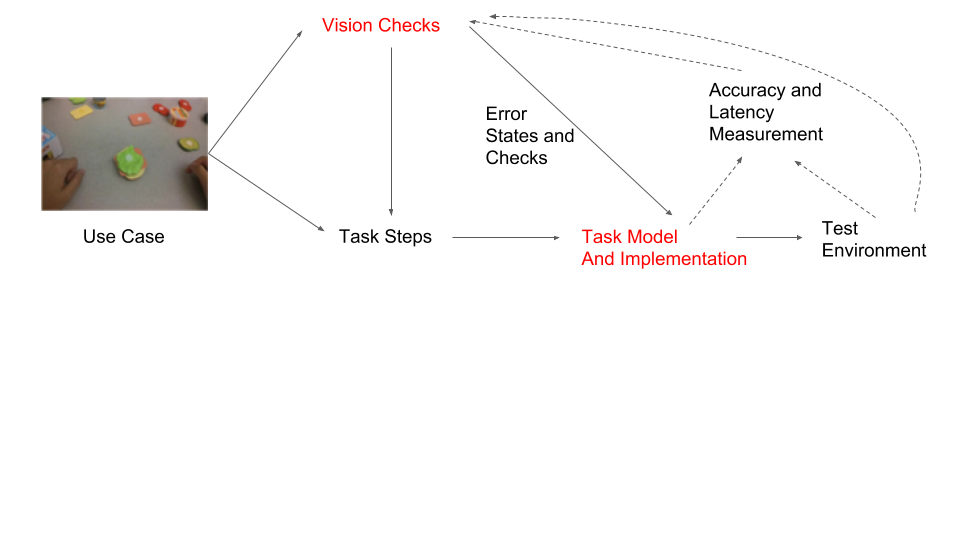
\includegraphics[trim={0 3in 0 0.2in},clip,width=7in]{FIGS/ad-hoc-workflow}
%% \caption{Ad-hoc Existing Workflow}
%% \label{fig:adhoc-workflow}
%% \end{figure}

Figure~\ref{fig:workflow} shows the ad-hoc development process. The most
critical step in building wearable cognitive assistance is to identify task
steps and the visual states of task steps. For example, for the Lego wearable
cognitive assistance ~\cite{chen2017empirical}, the task steps are the sequence
of shapes needed to achieve the final assembled lego shape. The visual states to
recognize are the current shapes on the lego board. Identifying visual states
and task steps takes significant time and expertise due to several reasons.
First, a developer needs to be familiar with the state-of-art of computer vision
algorithms to determine what visual states can be recognized reliably. Second,
identifying task steps requires domain knowledge. Third, when visual states
become too hard for CV, developers need to adjust the task steps to use other
methods for confirmation. Often a redesign of task steps is required to
compensate computer vision. For instance, when designing the RibLoc application,
a redesign of the task steps involves asking the user to read out a word on the
gauge instead of performing optical character recognition on the lightly-colored
characters.

I plan to work on building Gabriel development tools in my thesis. I want to
focus on providing automation tools for the most time-consuming procedures in
the development workflow -- building vision checks.

%% Object detection is at the core of computer vision tasks used by Gabriel
%% application. In Ping-Pong assistance, the Ping-Pong table, the ball, and the
%% opponent need to be recognized and localized. In Ikea Lamp assistance, the lamp
%% base, the shade, and the bulb need to be detected. Being able to create reliable
%% object detectors quickly can substantially facilitate application development.

%% Recent advances in
%% DNNs~\cite{girshick2014rich},~\cite{ren2015faster},~\cite{he2016deep} have not
%% only drastically improved the accuracy of object detection, but also provide an
%% opportunity to automate the creation of them. Unlike traditional CV algorithms,
%% DNNs adopt a end-to-end learning approach, in which features are no longer
%% hand-crafted but learned. The replacement of custom CV code with machine-learned
%% models gives automation opportunities. Nevertheless, creating a DNN-based object
%% detector is still both time-consuming and painstaking due to other reasons. DNNs
%% have a lot of parameters and requires millions of labeled examples to train from
%% scratch. Collecting and labeling these large amount of training data becomes a
%% bottleneck.

TPOD (Tool for Painless Object Detection) is a web-based tool I developed to
help quickly create DNN-based object detectors. It provides a tracking-assisted
labeling interface for speedy labeling and transfer learning-based DNN training
and evaluation backends that abstract the nuances of DNNs. Using TPOD to create
object detectors is straight-forward. A user would first upload short videos of
the object collected from varying lighting conditions and perspectives. Then,
the user would label these objects using TPOD's labeling interface. TPOD assists
labeling by tracking the labeled object across frames. Augmenting training data
with synthetically generated data is also supported. A user then can start training
from the web interface. TPOD backend uses transfer learning to finetune an
object detector DNN from publicly available networks that have been trained with
millions of images. When the training is done, a user can download the object
detector as a container image to run the trained models for inference. TPOD also
provides interfaces for evaluating and testing trained DNNs.

The initial prototype of TPOD has been used by researchers and students to build
wearable cognitive assistance. For example, a group of master students in CMU
mobile and pervasive computing class successfully used TPOD to build an
assistant for using AED machines.

Going forward, I plan to open-source the tool after following optimizations.
First, TPOD's backend needs to be easily extensible. With increasingly many
DNN-based object detectors developed in the computer vision community, adding a
new object detector to TPOD should be made easy. This design goal requires
well-modularized DNN backends with clean and easy-to-use interfaces to query
labeled datasets for training, standard serialization format to download, and
stable APIs to detect objects using the trained models. Second, TPOD's labeling
interface should be well isolated from the automated DNN training backend. With
such isolation, individuals looking for labeling tools can leverage TPOD's
front-end without setting up the training backend. This isolation requires
serializing labeled datasets using widely-used formats, for example, Pascal VOC
annotation format. Third, TPOD should be packaged well for installation. I plan
to containerize TPOD to make it easy for others to install.

\clearpage

%% \subsection{Automatic Workflow Extraction}

%% Identifying and implementing the task model in a wearble cognitive assistance
%% also takes a considerable amount time. In existing workflow, both these steps
%% are done manually with developers' domain knowledge, experience and intuition.
%% Automatic extraction of a workflow and generation of the task model
%% implementation can greatly reduce the development time.

%% Particularly, I will focus on mechanical assembly tasks since they often have
%% non-trivial number of steps and complex task model. I plan to work on automatic
%% extraction of workflow from videos. The inputs are videos recordings of correct
%% assembly procedures. The outputs are step sequences annotated with objects
%% involved for each step. Once the task model is extracted, a developer is able to
%% edit and add error states to complete the task model. In addition, I will strive
%% for building tools to generate code blocks from a task model.

% \section{Timeline}

\begin{table}[ht]
\centering
\begin{tabular}{ccc}
\toprule[1pt]\midrule[0.3pt]
\multicolumn{2}{c}{Timeline}                                                                                           & Plan                                                                                                 \\ \hline
\multicolumn{1}{c|}{2018 Summer} & \multicolumn{1}{c|}{May - Aug}                                                      & Apply Bandwidth Reduction to Gabriel Applications                                         \\ \hline
\multicolumn{1}{c|}{2018 Fall}   & \multicolumn{1}{c|}{\begin{tabular}[c]{@{}c@{}}Sept - Nov\\       Dec\end{tabular}} & \begin{tabular}[c]{@{}c@{}}Complete Gabriel Acceleration Framework\\ MobiSys submission\end{tabular} \\ \hline
\multicolumn{1}{c|}{2019 Spring} & \multicolumn{1}{c|}{\begin{tabular}[c]{@{}c@{}}Jan - April\\ May\end{tabular}}      & \begin{tabular}[c]{@{}c@{}}Build Gabriel Development Tools\\ SEC submission\end{tabular}             \\ \hline
\multicolumn{1}{c|}{2019 Summer} & \multicolumn{1}{c|}{May - Aug}                                                      & Thesis Writing                                                                                       \\ \hline
\multicolumn{1}{c|}{2019 Fall}   & \multicolumn{1}{c|}{\begin{tabular}[c]{@{}c@{}}Sept - Nov\\ Dec\end{tabular}}       & \begin{tabular}[c]{@{}c@{}}Finish thesis dissertation\\ Thesis Defense\end{tabular}                  \\ \midrule[0.3pt]\bottomrule[1pt]
\end{tabular}
\end{table}

% {\let\clearpage\relax \section{Related Work}}

\subsection{Edge Computing}

Gabriel applications offload computation to a cloudlet, a small data-center at
the edge of the internet~\cite{satyanarayanan2009case}. The high bandwidth and
low latency offered by cloudlets~\cite{ha2013impact}~\cite{hu2016quantifying}
lay the foundation of wearable cognitive assistance~\cite{ha2014towards}.
Previous research has worked on VM synthesis~\cite{ha2013just} to enable rapid
provisioning of applications onto a cloudlet. In addition, user mobility is
supported through VM handoff~\cite{ha2017you}, which migrates user states from
one cloudlet to another. These pioneer work into cloudlet together with
decade-long research into computational
offload~\cite{cuervo2010maui}~\cite{gordon2012comet}~\cite{flinn2012cyber}
provides the infrastructure support that makes wearable cognitive assistance
applications feasible. Previous measurement of edge computing's impact on mobile
applications tested compute-intensive and latency-sensitive applications when
network utilization is low~\cite{chen2017empirical}. This work relaxes such assumption and
focuses on supporting more users when the resource utilization is high.

\subsection{Cognitive Assistance Applications}
This work builds on top of existing efforts into creating wearable cognitive
assistance~\cite{ha2014towards}~\cite{chen2015early}~\cite{chen2017empirical}.
While previous work has focused on identifying latency requirements and system
optimizations to meet latency constraints, this work focuses on making wearable
cognitive assistance economically feasible. Other earlier works have also
explored providing cognitive assistance to users. For instance,
~\cite{loomis1998navigation} created a navigation system for the blind twenty
years ago. Rhema~\cite{tanveer2015rhema} used Google Glass to help people with
public speaking. ~\cite{williams2015designing} provided people with aphasia
conversational cues on a head-worn display.

Most of these applications run solely on mobile devices and are highly
constrained by the limited compute budget. Gabriel applications use an offload
approach to leverage beefy static computational resources. Gabriel applications
can use state-of-art DNN-based computer vision algorithms to perform
complex CV tasks.

\subsection{Mobile System Support for Computer Vision Workload}
With the proliferation of smartphones and cameras, many research works have
studied mobile system supports for computer vision workload.
~\cite{likamwa2015starfish} designed and built a system to efficiently support
many concurrent computer vision applications on a mobile device.
~\cite{lane2015zoe} built a custom wearable device that supports continuous
inference on sensor data using a low power budget. More recently, many more
efforts have been focused on DNNs. ~\cite{yao2017deepsense} and
~\cite{huynh2017deepmon} accelerated DNN inference on commodity mobile GPUs.
~\cite{han2016mcdnn} looked at where to schedule DNNs of different
accuracy and speed tradeoff under resource constraints.
~\cite{likamwa2016redeye} executed convolutional layers in analog domain before
sensor read-out to reduce power consumption.

Besides, many researchers have worked on algorithmic optimizations to reduce
DNN computation. ~\cite{han2015deep}~\cite{iandola2016squeezenet} compressed DNN
models by pruning insignificant weights. ~\cite{han2016eie} showcased a DNN
hardware accelerator exploiting model compression techniques.
~\cite{wu2016quantized}~\cite{gong2014compressing} studied weight quantization
for faster inference. ~\cite{howard2017mobilenets}~\cite{sandler2018inverted} designed DNNs with
depth-wise separable convolutions to decrease DNN parameters and increase
inference speed on mobile devices.

While Gabriel applications can benefit from improvement on mobile system support
for DNNs, we recognize the lasting trend in the performance gap between mobile
devices and static elements. The offload approach we adopt enables us to
leverage powerful computational resources at the edge of the internet. The
improvement in mobile system support for DNNs can help us build better early
discard filters and perform more dynamic adaptation to user context.

%\appendix
%\include{appendix}

\backmatter

%\renewcommand{\baselinestretch}{1.0}\normalsize

% By default \bibsection is \chapter*, but we really want this to show
% up in the table of contents and pdf bookmarks.
\renewcommand{\bibsection}{\chapter{\bibname}}
%\newcommand{\bibpreamble}{This text goes between the ``Bibliography''
%  header and the actual list of references}
\bibliographystyle{plainnat}
\bibliography{proposal} %your bib file

\end{document}
